\documentclass[VM.tex]{subfiles}
\tikzset{
  load/.style   = {ultra thick,-latex},
  stress/.style = {-latex},
  dim/.style    = {latex-latex},
  axis/.style   = {-latex,black!55},
}

% Drawing View
\tikzset{dimetric2/.style={
  x={(0.935cm,-0.28cm)},
  y={(0.44cm, 0.312cm)},
  z={(0.000cm, 0.943cm)},
}}
\begin{document}

\subsubsection*{Description : }
A simply Supported square plate with distributed load (q). 
\subsubsection*{Reference : }
S.Timoshenko , S . Woinowsky , Theory of Plates and Shells , pg:116, Article : 30 . \\

\subsubsection*{Material and Geometric data : }


\begin{figure}[h!]
\centering
\subfile{TIM116_DRAW.tex}
\caption{TIM116} \label{TIM116sch}
\end{figure}
\begin{table}[h!]
\renewcommand{\arraystretch}{1.5}
\centering
\caption{Input Data}
\label{my-labelsdqf}
\begin{tabular}{|ll|ll|ll|}
\hline
\multicolumn{2}{|l|}{\cellcolor[HTML]{C0C0C0}Material Property} & \multicolumn{2}{l|}{\cellcolor[HTML]{C0C0C0}Geometric Data} & \multicolumn{2}{l|}{\cellcolor[HTML]{C0C0C0}Loading Data} \\ \hline  \hline
Young's Modulus ($E$)          & 2E11 $pa$         & Length ($a$)        & 10 $m$        &      Distributed Load ($q$)  & 1000 $N/m^2$     \\
Poission's Ratio ($\nu$)       & 0.3         & Breath ($b$)        & 10 $m$          &        &      \\ 
    &         & Thickness($t$)        & 0.1 $m$          &    &        \\ \hline
\end{tabular}
\end{table}




\subsubsection*{Mesh and boundary condition : }



\begin{figure}[h!]
\begin{subfigure}{.45\textwidth}
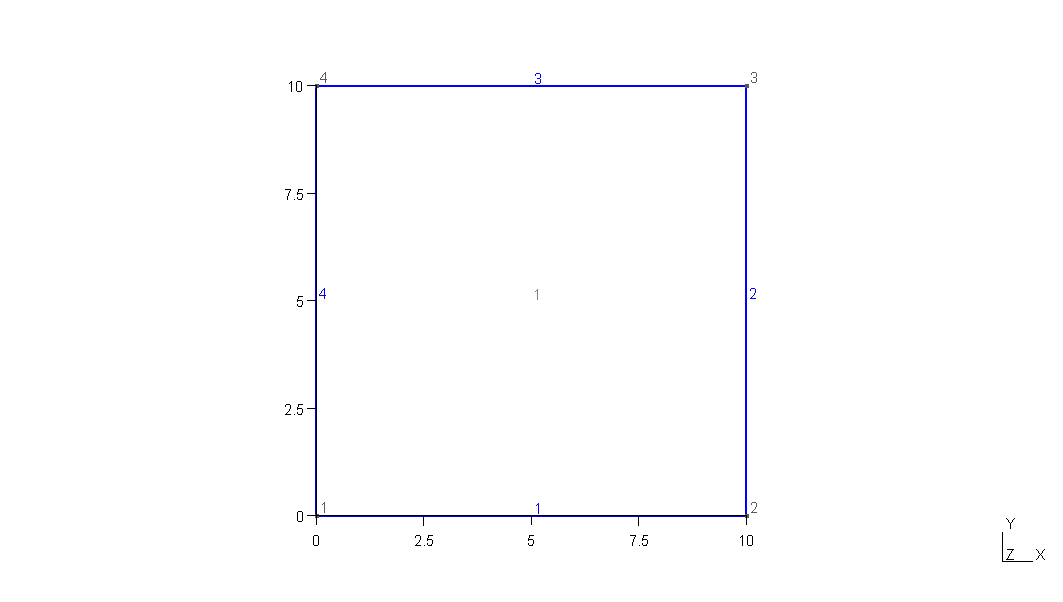
\includegraphics[width=\linewidth,trim={8cm 0 8cm 0},clip]{TIM116/TIM116_geo.png}
%\caption{Mode Shape 4}
\end{subfigure} \hfill
\begin{subfigure}{.45\textwidth}
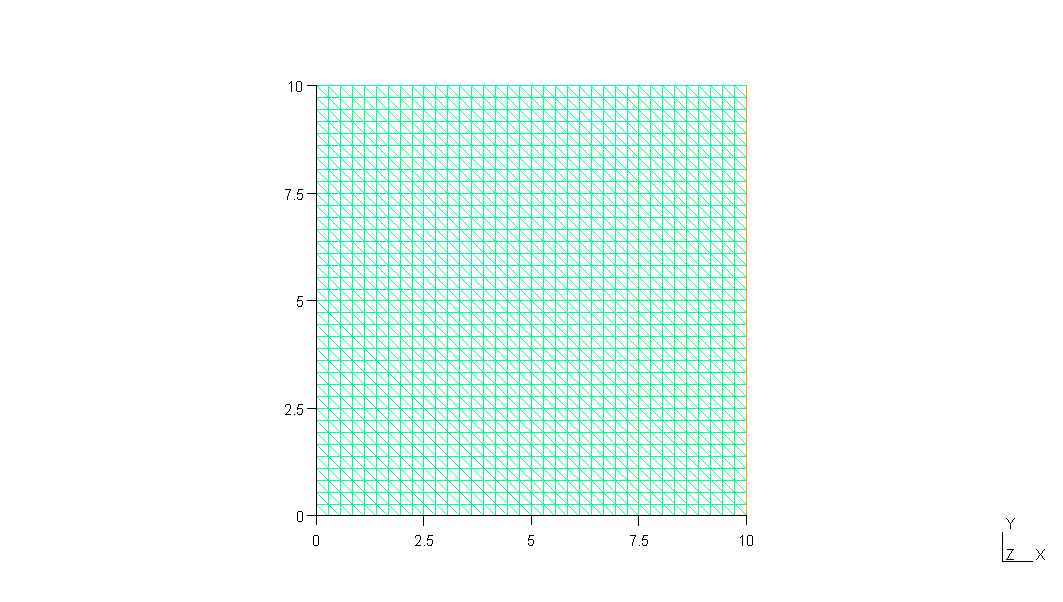
\includegraphics[width=\linewidth,trim={8cm 0 8cm 0},clip]{TIM116/TIM116_msh.png}
%\caption{Mode Shape 5}
\end{subfigure}
\caption{Geomentry and Mesh of TIM116}
\end{figure}







\begin{table}[h!]
\renewcommand{\arraystretch}{1.5}
\centering
\caption{FEM and Boundary condition data}
\label{my-label}
\begin{tabular}{|l|lll|l|lll|}
\hline
 \multicolumn{4}{l|}{\cellcolor[HTML]{C0C0C0}Direchlet Boundary} & \multicolumn{4}{l|}{\cellcolor[HTML]{C0C0C0}Neumann Boundary} \\ \hline \hline
Geo - \newline Entity      & $w$          & $\theta _ x$     & $\theta _ y $    & Geo - \newline Entity         & $F_z$        & $M_x$        & $M_y$        \\    
                 line \{1,2,3,4\}                   & Fixed      & Free         & Free        & Area \{1\}                    & 1000 $N/m^2$        &           &          

 \\ \hline
\end{tabular}
\end{table}
\subsubsection*{Analytically solution : }
The $w_{max}$which is the w displacement at the middle of the plate is given by
\begin{equation}
w_{max}=0.00406 \frac{qb^4}{D}
\end{equation}


The analytically solution of the problem is calculated as $w_{max} =-0.0022167 m $

\subsubsection*{Result and error analysis : }

\begin{figure}[h!]
\centering
\minipage{1\textwidth}%
  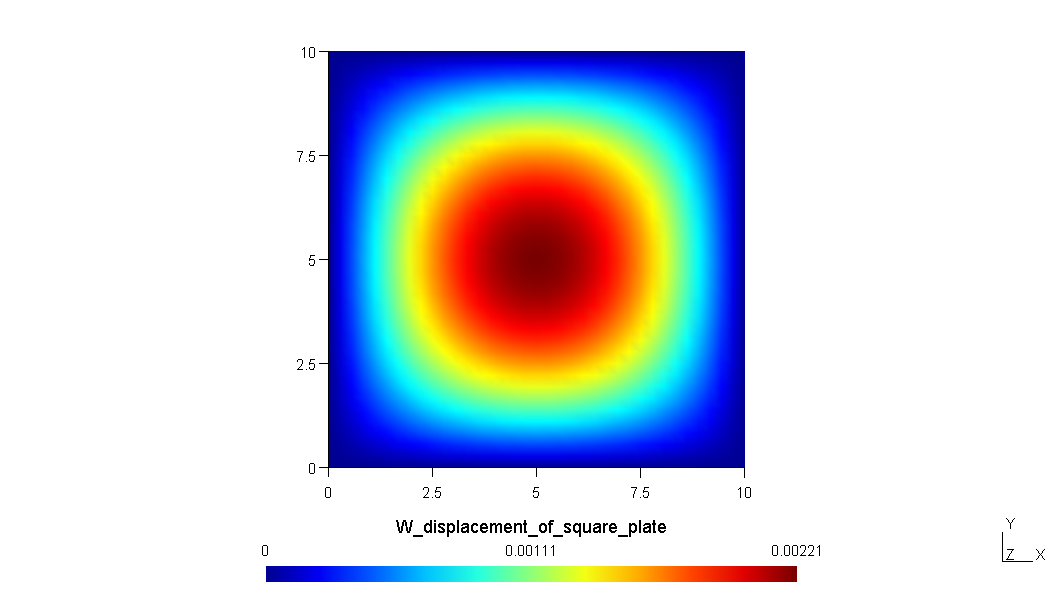
\includegraphics[width=\linewidth,trim={8cm 0 8cm 0},clip]{TIM116/TIM116_pos.png}
  \caption{FEM solution plot}\label{fig:awesome_image3}
\endminipage
\end{figure}
The maximum displacement of the domain is our solution . w displacement at middle is $ -0.0022144 m $.


\begin{equation}
error \% = \mid \frac{w_{analytical}-w_{FEM}}{w_{analytical}} \mid \times 100
\end{equation}

So the Error percentage is $ 0.1 \% $. 

\end{document}